\documentclass[aspectratio=169, lualatex]{beamer} %, handout
\makeatletter\def\input@path{{theme/}}\makeatother\usetheme{cipher}

\title{Computer Security: Post Quantum Security}
\author{Markulf Kohlweiss}
\subject{Introduction to Applied Cryptography covering cryptographic primitives, protocols, security goals, and real-world applications from basic concepts to advanced topics like TLS and zero-knowledge proofs.}
\keywords{cryptography, security, encryption, authentication, hash functions, TLS, protocols, provable security}
\institute{University of Edinburgh, School of Informatics}
\instituteimage{images/edu-white.png}
\date{\today}
\coversubtitle{INFR10067\\Fall 2025}
\coverpartname{Cryptography}
\covertopicname{Post-Quantum Security}
\coverwebsite{}

\usepackage[absolute,overlay]{textpos} % put in preamble

\colorlet{gris}{black!50!white}
\def\engris#1{\textcolor{gris}{#1}}

\colorlet{jaune}{yellow!90!black}
\def\enjaune#1{\textcolor{jaune!70!black}{#1}}

\colorlet{vert}{green!45!black}
\def\envert#1{\textcolor{vert}{#1}}

\colorlet{bleu}{blue!70!black}
\def\enbleu#1{\textcolor{bleu}{#1}}

\colorlet{rouge}{red!75!black}
\def\enrouge#1{\textcolor{rouge}{#1}}

\newcommand{\rouge}{\only{\color{rouge}}}

\xdefinecolor{violet}{rgb}{.5,0,.7}
\def\enviolet#1{\textcolor{violet}{#1}}

\xdefinecolor{violetft}{rgb}{0.199,0., 0.398}
\def\envioletft#1{\textcolor{violetft}{#1}}

\xdefinecolor{monbleu}{rgb}{0,.2,.54}
\newcommand{\monbleu}{\only{\color{monbleu}}}

\begin{document}
\begin{frame}[plain]
	\titlepage
\end{frame}

\begin{frame}{Recap}
	\vspace{-0.5cm}

  Action items:
  \begin{itemize}
  \item[$\checkmark$] Upload slides in advance
\item[?] Question: DNSSEC vs Certs. DANE vs PKI? \envert{\footnotesize-- DNS-based Authentication of Named Entities} \\ \pause
{\footnotesize\url{www.ipfire.org/blog/global-pki-considered-harmful-a-plaidoyer-for-using-dane}}\pause
  \item[?] Question: Can quantum computers solve NP-hard problems? \envert{No and a little yes} \\ {\footnotesize Grover's algorithm provides a quadratic speedup for unstructured search. \\ \envert{Does not change the fundamental complexity class.}} \pause 
  \item[?] Exercises: Those that struggle, did you read the short chapter and do the exercises here: \url{https://joyofcryptography.com/pdf/chap0.pdf}? \smallskip \pause
  \item[$\checkmark$] \textbf{Office hours} are 11:15 Mon and Fri. 
  {\footnotesize Talk with me after lecture, also BSc students. \\ 
Specialization, e.g., Blockchain \& Distributed Ledgers, Security and Privacy for AI, Zero Knowledge.} \envert{Guest Lecture, Friday 31st of October.}\pause
  \item[$\checkmark$] Request: Challenges in modern cryptography?  
  %Trusted, distributed, fair and safe AI. Digital and Decentralized Identity. 
  Post-quantum. \textbf{Protocols} \\ {\footnotesize Formalization of cryptography and \emph{protocols} in theorem provers, e.g. Lean.}
  \end{itemize}

  We finished "Why Go Post-Quantum?" and are at "Going Post-Quantum".

\end{frame}

\section{Why Go Post-Quantum?}

\begin{frame}{The quantum threat}
	\begin{itemize}
		\item \textbf{Quantum computers} are fundamentally different from classical computers
		\item They exploit quantum mechanical phenomena: 
		
		\begin{center}\envert{superposition, entanglement, and interference}
		\end{center}\pause
		\item Can solve certain problems exponentially faster than classical computers \\
		\envert{and other problems faster but not exponentially faster}\pause
		\item \textbf{Critical insight}: Many cryptographic algorithms rely on problems that quantum computers could solve efficiently
	\end{itemize}
\end{frame}

\begin{frame}{How quantum computers work}
	\begin{itemize}
		\item \textbf{Classical bits}: Can be either 0 or 1
		\item \textbf{Quantum bits (qubits)}: Can be in \textit{superposition} of 0 and 1 simultaneously
		\item \textbf{Superposition}: A qubit can represent both states at once \envert{(rough intuition)}
		      \begin{itemize}
			      \item $n$ classical bits: Store one of $2^n$ possible values
			      \item $n$ qubits: Can represent all $2^n$ values simultaneously
		      \end{itemize}\pause
		\item \textbf{Entanglement}: Qubits can be correlated in ways impossible classically
		      \begin{itemize}
			      \item Measuring one qubit instantly affects others
			      \item Enables parallel computation across exponentially many states
		      \end{itemize}
		\item \textbf{Quantum parallelism}: Process all possibilities at once, extract answer through interference \pause
		
\envert{Misunderstanding that quantum computers can “try all solutions instantly.” The reality is more nuanced, yet still revolutionary.}
	\end{itemize}
\end{frame}

\begin{frame}{Wikipedia visualization of interference: no interference}
	\bigimagewithcaption{interference-off.png}{Source: Wikipedia for Mach-Zehnder interferometer}
\end{frame}

\begin{frame}{Wikipedia visualization of interference: interference}
	\bigimagewithcaption{interference-on.png}{Source: Wikipedia for Mach-Zehnder interferometer}
\end{frame}

\begin{frame}{Building quantum computers: the engineering challenge}
	\begin{itemize}
		\item \textbf{Multiple approaches being pursued}:
		      \begin{itemize}
			      \item Superconducting circuits (IBM, Google)
			      \item Trapped ions (IonQ, Honeywell)
			      \item Topological qubits (Microsoft)
			      \item Photonic qubits (Xanadu, PsiQuantum)
			      \item Neutral atoms (QuEra, Pasqal)
		      \end{itemize}
		\item \textbf{Common requirement}: Maintain quantum coherence
		      \begin{itemize}
			      \item Qubits must remain in superposition
			      \item \enrouge{Any interaction with environment causes \textit{decoherence}}
			      \item Current coherence times: microseconds to milliseconds
		      \end{itemize}
	\end{itemize}
\end{frame}

\begin{frame}{Physical challenges: Why qubits are so difficult}
	\begin{itemize}
		\item \textbf{Size requirements}: Qubits are difficult to physically manipulate
		      \begin{itemize}
			      \item Individual photons, electrons, or atomic nuclei
			      \item Some approaches (superconducting) have larger qubits
			      \item Impossible to manipulate with conventional tools
			      \item Require laser beams or electromagnetic fields for control
		      \end{itemize}
		\item \textbf{Temperature requirements}: Near absolute zero (-273\degree\ C)
		      \begin{itemize}
			      \item For some quantum systems, tiny amounts of heat destroy quantum states
			      \item Requires dilution refrigerators costing millions
			      \item More cooling power needed as system scales
		      \end{itemize}
		\item \textbf{Isolation from environment}:
		      \begin{itemize}
			      \item Magnetic fields, vibrations, cosmic rays all cause errors
			      \item Need multiple layers of shielding
			      \item Even observation destroys quantum states! \enrouge{(observation = interaction)}
		      \end{itemize}
	\end{itemize}
\end{frame}

\begin{frame}{The coherence problem: Racing against time}
	\begin{itemize}
		\item \textbf{Coherence time}: How long qubits maintain their quantum state
		      \begin{itemize}
			      \item Current record: A few seconds at best
			      \item Most systems: Microseconds to milliseconds
			      \item Breaking crypto needs: Days to weeks of computation
		      \end{itemize}
		\item \textbf{Error rates}: Quantum operations are inherently noisy
		      \begin{itemize}
			      \item Classical computers: 1 error per $10^{17}$ operations
			      \item Current quantum computers: 1 error per $10^{3}$ operations
			      \item Need massive improvement to be useful
		      \end{itemize}
		\item \textbf{Quantum error correction}:
		      \begin{itemize}
			      \item Can't copy quantum states (no-cloning theorem)
			      \item Need 100-1000 physical qubits to make 1 logical qubit
			      \item \enrouge{Turns ``millions of qubits'' requirement into ``billions of physical qubits'' requirement}
		      \end{itemize}
	\end{itemize}
\end{frame}

\begin{frame}{What makes current cryptography vulnerable?}
	\begin{itemize}
		\item \textbf{RSA}: Based on factoring large integers
		\item \textbf{Diffie-Hellman}: Based on discrete logarithm problem (DLP)
		\item \textbf{Elliptic Curve Cryptography (ECC)}: Also based on DLP but over different group
		\item These are \textit{hard} for classical computers but \textit{easy} for quantum computers
		\item \textbf{Shor's algorithm} (1994): Polynomial-time quantum algorithm for factoring and discrete log
		\item \textbf{Grover's algorithm} (1996): Sub-exponential quantum algorithm for search affecting symmetric cryptography
	\end{itemize}
\end{frame}

\begin{frame}{Grover's algorithm: summary}
	\begin{itemize}
		\item \textbf{Grover's algorithm}: Quantum algorithm for searching unsorted databases
		\item \textbf{Classical search}: $\mathcal{O}(2^n)$ time to search $2^n$ items \pause
		\item \textbf{Quantum search}: $O(2^{n/2})$ time with Grover's algorithm \pause
		\item \textbf{Formal claim}: Given $F: \{0,1\}^n \rightarrow \{0,1\}$, Grover's algorithm makes $O(2^{n/2})$ quantum evaluations of $F$ and outputs $X \in \{0,1\}^n$ such that $F(X) = 1$, if such $X$ exists \pause
		\item \textbf{Intuition}: Finding needles in haystacks
		      \begin{itemize}
			      \item Haystack: $\{0,1\}^n$ (all possible inputs)
			      \item Needle: Special input $X$ where $F(X) = 1$
		      \end{itemize}
	\end{itemize}
\end{frame}

\begin{frame}{Grover's algorithm: attacking symmetric cryptography}
	\begin{columns}[c]
		\begin{column}{1\textwidth}
			\begin{itemize}
				\item \textbf{Attack setup}: Obtain known plaintext-ciphertext pairs for key $K$ of lenght $k$
				      \begin{itemize}
					      \item $C_1 = \text{Enc}(K, M_1)$, $C_2 = \text{Enc}(K, M_2)$, ..., $C_m = \text{Enc}(K, M_m)$
				      \end{itemize}
				\item \textbf{Define search function}:
				      \begin{align*}
					      F(K) = \begin{cases}
						             1 & \text{if } \text{Dec}(K, C_i) = M_i \text{ for all } i \\
						             0 & \text{otherwise}
					             \end{cases}
				      \end{align*}\pause
				\item \textbf{Result}: Grover finds the correct key in $O(2^{k/2})$ time%\footnote{Note: Grover's algorithm is inherently sequential (cannot be parallelized efficiently)}
				\item \textbf{Defense}: Double the key size %\footnote{Cryptographers argue about this recommendation in different points, some thinking it's too simplistic, others thinking that with hash functions, you may not need to go from SHA-256 to SHA-512 with SHA-384 being enough, etc.}
				      \begin{itemize}
					      \item AES-128 $\rightarrow$ AES-256 (to maintain 128-bit security)
					      \item SHA-256 $\rightarrow$ SHA-512 (for collision resistance)
				      \end{itemize}
			\end{itemize}
		\end{column}
	\end{columns}
\end{frame}

\begin{frame}{Shor's algorithm: summary}
	\begin{itemize}
		\item In 1994, Peter Shor demonstrated that quantum computers could break most asymmetric-key cryptography in polynomial time
		\item \textbf{Claim}: There are quantum algorithms for the following tasks, whose running time is polynomial in $k$:
		      \begin{itemize}
			      \item Factoring $k$-bit numbers
			      \item Solving the discrete logarithm problem in any cyclic group of order $< 2^k$, even groups based on elliptic curves
		      \end{itemize}
		\item Both algorithms use a common approach called \textit{Shor's algorithm}
		\item \textbf{Implication}: All public-key cryptography based on factoring (RSA) or discrete logarithm (Diffie-Hellman, ElGamal, Schnorr) can be broken by quantum computers
	\end{itemize}
\end{frame}

\iffalse
\begin{frame}{Shor's algorithm: impact}
	\begin{columns}[c]
		\begin{column}{0.5\textwidth}
			\begin{itemize}
				\item Classical factoring: Known algorithms take sub-exponential time
				\item Quantum factoring with Shor's: Takes polynomial time
				\item Example: Factoring a 2048-bit RSA key
				      \begin{itemize}
					      \item Classical: Billions of years
					      \item Quantum: Hours to days (with a large enough quantum computer)
				      \end{itemize}
				\item \textbf{Impact}: Complete break of RSA, ECC, and DH key exchange
			\end{itemize}
		\end{column}
		\begin{column}{0.5\textwidth}
			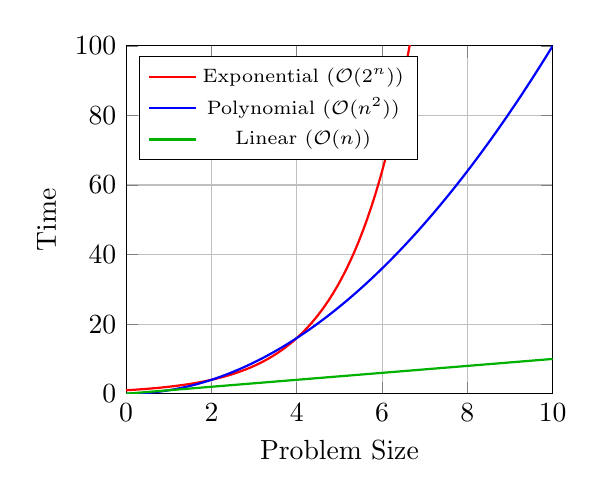
\begin{tikzpicture}[scale=1]
				\begin{axis}[
						xlabel={Problem Size},
						ylabel={Time},
						xmin=0, xmax=10,
						ymin=0, ymax=100,
						legend pos=north west,
						legend style={font=\scriptsize, align=left},
						grid=major,
						width=7cm,
						height=6cm,
					]
					\addplot[red, thick, domain=0:10, samples=100] {2^x};
					\addlegendentry{Exponential ($\mathcal{O}(2^n)$)}
					\addplot[blue, thick, domain=0:10, samples=100] {x^2};
					\addlegendentry{Polynomial ($\mathcal{O}(n^2)$)}
					\addplot[green!70!black, thick, domain=0:10] {x};
					\addlegendentry{Linear ($\mathcal{O}(n)$)}
				\end{axis}
			\end{tikzpicture}
		\end{column}
	\end{columns}
\end{frame}
\fi

\begin{frame}{Not all cryptography is equally vulnerable}
	\begin{columns}[c]
		\begin{column}{1\textwidth}
			\begin{itemize}
				\item \textbf{Asymmetric cryptography}: Severely impacted by quantum computers
				      \begin{itemize}
					      \item RSA, Elliptic Curve Cryptography (ECC), DH $\rightarrow$ \enrouge{Broken by Shor's algorithm}
				      \end{itemize}\pause
				\item \textbf{Symmetric cryptography}: Less impacted
				      \begin{itemize}
					      \item AES, SHA-256 $\rightarrow$ Weakened but not broken
					      \item \enrouge{Grover's algorithm: Provides quadratic speedup}
					      \item Solution: Double the key size \envert{(AES-128 $\rightarrow$ AES-256)}%\footnote{Cryptographers argue about this recommendation in different points, some thinking it's too simplistic, others thinking that with hash functions, you may not need to go from SHA-256 to SHA-512 with SHA-384 being enough, etc.}
				      \end{itemize}\pause
				\item \textbf{Hash functions}: Similar to symmetric crypto
				      \begin{itemize}
					      \item Need larger output sizes to maintain security \envert{(SHA-256 $\rightarrow$ SHA-512)}
				      \end{itemize}
			\end{itemize}
		\end{column}
	\end{columns}
\end{frame}

\begin{frame}{Timeline: when will quantum computing arrive?}
	\begin{itemize}
		\item \textbf{Current state}: Small quantum computers exist (100s of qubits)
		\item \textbf{Required for cryptanalysis}: Millions of error-corrected qubits
		\item \textbf{Expert predictions}: 10-30 years until cryptographically relevant quantum computers (depending on who you ask)
		\item \textbf{But consider}:
		      \begin{itemize}
			      \item Technological breakthroughs could accelerate timeline
			      \item Nation-states investing billions in quantum research
			      \item Progress has been faster than expected in recent years
		      \end{itemize}
	\end{itemize}
\end{frame}

\begin{frame}{Timeline: when will quantum computing arrive?}{ Billion dollar question}
\vspace{-0.7cm}
	\begin{figure}[c]
		\centering
	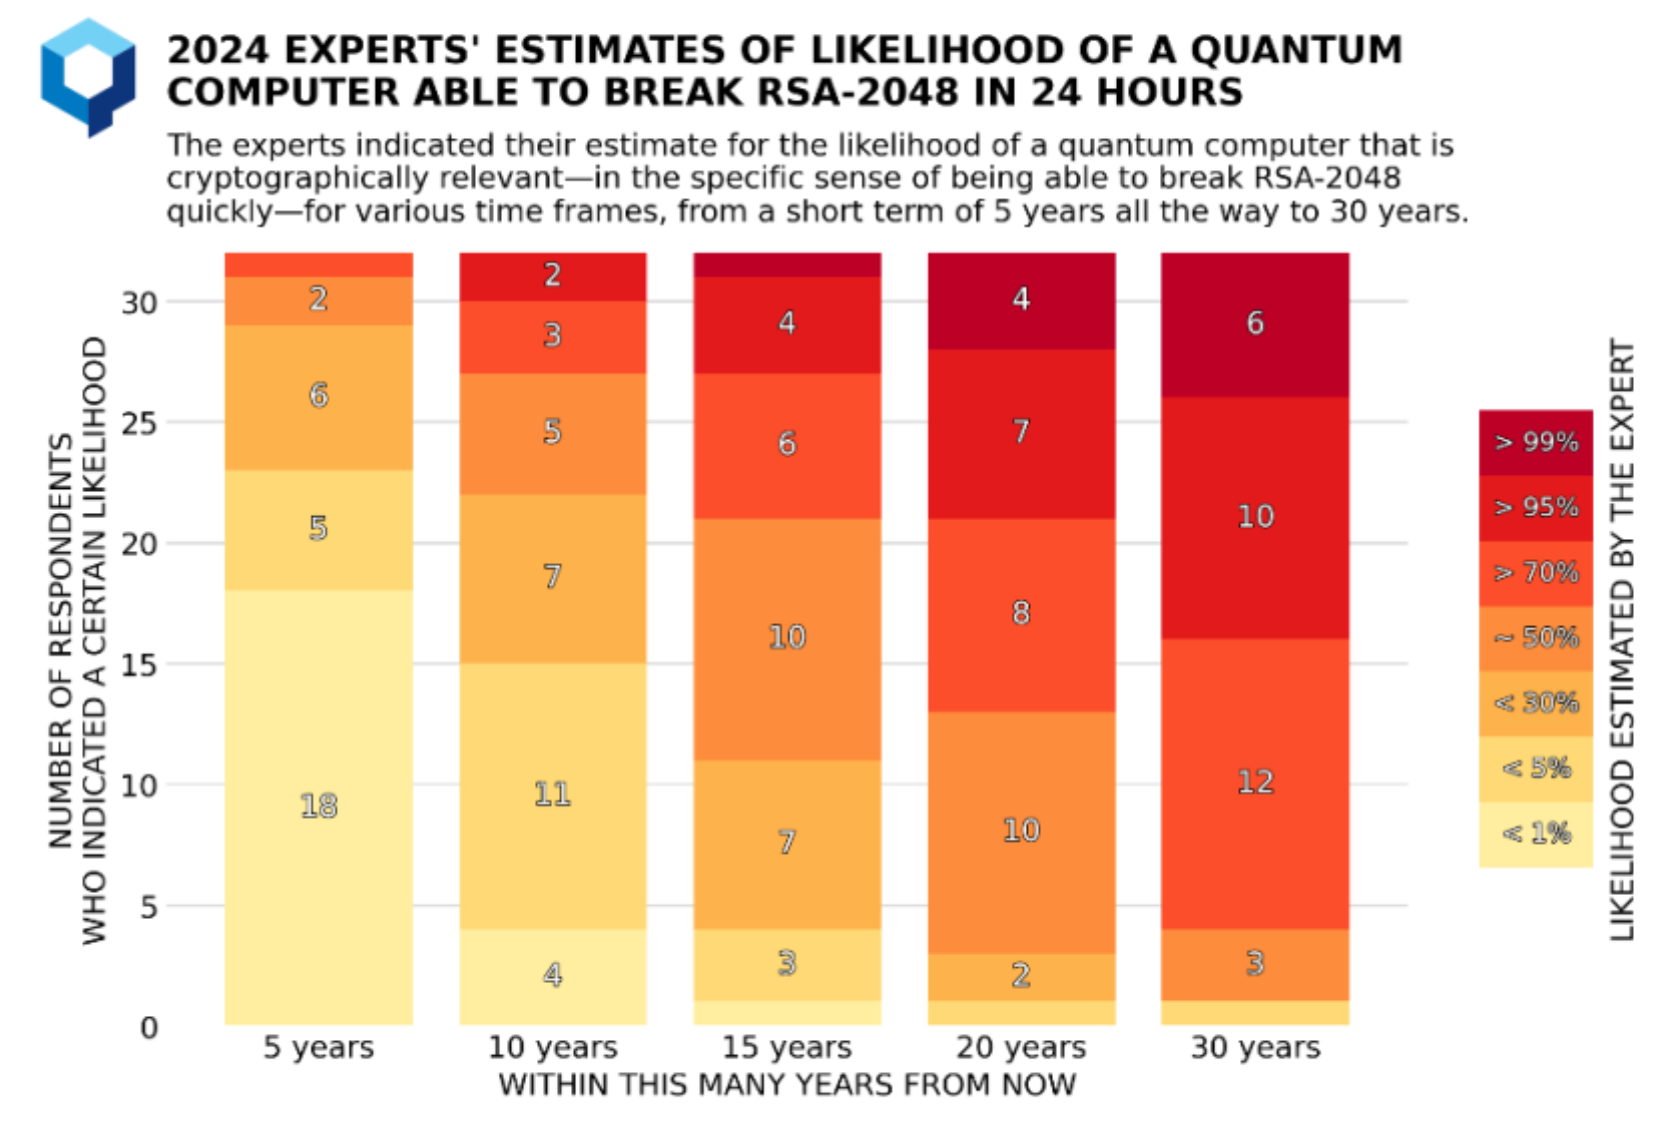
\includegraphics[scale=0.16]{images/quantum-threat.png}
	\vspace{-0.4cm}
	\caption{Source: Michele Mosca and Marco Piani, Quantum Threat Timeline Report, Global Risk Institute, 2024.}
	\end{figure}
\end{frame}

\begin{frame}{Timeline: will we still be alive to witness arrival?}{Life or death question}
	\vspace{-0.7cm}
		\begin{figure}[c]
		\centering
	\includegraphics[scale=0.46]{images/worldwar.png}
	\vspace{-0.4cm}
	\caption{\url{https://yougov.co.uk/politics/articles/48527-world-war-3-likely-in-next-5-10-years-think-most-britons}}
	\end{figure}
\end{frame}

\begin{frame}{Timeline: according to Sam Jaques}
	\bigimagewithcaption{quantum-timeline.png}{Source: Sam Jaques}
\end{frame}

\begin{frame}{Reality check: Current quantum factorization records}
	\begin{itemize}
		\item \textbf{2001}: IBM factored $15 = 3 \times 5$ using Shor's algorithm
		\item \textbf{2012}: Factored $21 = 3 \times 7$
		\item \textbf{2019}: Attempted to factor $35 = 5 \times 7$
		\item \textbf{In 24 years}: Progress from 15 to 21
		\item \textbf{For context}: A 1981 VIC-20 home computer can factor these numbers instantly
		\item These aren't even true applications of Shor's algorithm - they use ``compiled'' versions with prior knowledge of the answer
	\end{itemize}
\end{frame}

\begin{frame}{Alternative ``quantum'' factorization methods}
	\begin{columns}[c]
		\begin{column}{1\textwidth}
			\begin{itemize}
				\item Recent paper\footnote{\url{https://appliedcryptography.page/paper/\#quantum-dog}} demonstrates matching all quantum factorization records using:
				      \begin{itemize}
					      \item \textbf{VIC-20}: 8-bit computer from 1981 (538 bytes of code)
					      \item \textbf{Abacus}: Ancient counting device
					      \item \textbf{Dog}: Trained to bark 3 times (factors 15 and 21)
				      \end{itemize}
				\item All methods successfully factor every number claimed by quantum computers
		%		\item The VIC-20 can factor the RSA-2048 ``quantum'' examples in 16.5 seconds
				\item \textbf{Conclusion}: Current quantum computers offer no practical advantage
			\end{itemize}
		\end{column}
	\end{columns}
\end{frame}

\iffalse
\begin{frame}{The sleight-of-hand problem}
	\begin{itemize}
		\item Most quantum factorization claims use specially constructed ``sleight-of-hand'' numbers
		\item \textbf{Example}: RSA-2048 ``factorization'' claims
		      \begin{itemize}
			      \item Factors chosen to differ by only 2 or 6
			      \item Real RSA keys require factors to differ by >100 bits
			      \item Can be factored with simple square root calculation
		      \end{itemize}
		\item \textbf{Common tricks}:
		      \begin{itemize}
			      \item Numbers with special binary patterns (mostly zeros)
			      \item Preprocessing on classical computers
			      \item ``Compiled'' algorithms that know the answer in advance
		      \end{itemize}
	\end{itemize}
\end{frame}

\begin{frame}{The gap between hype and reality}
	\begin{itemize}
		\item \textbf{Claimed}: ``RSA-2048 factored by quantum computer''
		\item \textbf{Reality}: Used specially constructed weak keys, solvable on 1980s hardware
		\item \textbf{Estimated timeline}: 10-30 years to cryptographically relevant quantum computers
		\item \textbf{Historical note}: Similar timeline estimates have been made for decades
		\item \textbf{Critical question}: Should we redesign all cryptography based on devices that can't outperform a dog?
	\end{itemize}
\end{frame}

\fi

\begin{frame}{Store now, decrypt later}
	\begin{itemize}
		\item \textbf{The problem}: Adversaries can store encrypted data today
		\item Wait for quantum computers to become available
		\item Decrypt all previously recorded communications
		\item \textbf{Implications}:
		      \begin{itemize}
			      \item Data encrypted today may be decrypted in 10-20 years
			      \item Long-term secrets are already at risk
			      \item Medical records, government communications, trade secrets
		      \end{itemize}
		\item \textbf{This attack is happening NOW}
		\item This is why some argue that we can't just not do anything because quantum computers seem impractical \textit{today}
	\end{itemize}
\end{frame}

\begin{frame}{Real-world impact: who needs to care?}
	\begin{itemize}
		\item \textbf{Financial institutions}: Protecting transactions and customer data
		\item \textbf{Healthcare}: Medical records must remain private for decades
		\item \textbf{Government}: National security and citizen privacy
		\item \textbf{Technology companies}: Secure communications and data storage
		\item \textbf{Critical infrastructure}: Power grids, water systems, transportation
		\item \textbf{Everyone}: Personal communications, passwords, private data
	\end{itemize}
\end{frame}

\begin{frame}{Why transition now?}
	\begin{itemize}
		\item \textbf{Migration takes time}: Historical crypto transitions took 10-20 years
		      \begin{itemize}
			      \item Recall the transition away from RC4, seen earlier in the course!
		      \end{itemize}
		\item \textbf{Complex systems}: Need to update protocols, libraries, hardware
		\item \textbf{Backward compatibility}: Must support both old and new systems
		\item \textbf{Unknown vulnerabilities}: New algorithms need time for analysis
		\item \textbf{Compliance and standards}: Regulations take years to update
		\item \textbf{Bottom line}: If we wait until quantum computers exist, it's too late
	\end{itemize}
\end{frame}

\section{Going Post-Quantum}

\begin{frame}{Post-quantum cryptography: the solution}
	\begin{itemize}
		\item \textbf{Definition}: Cryptographic algorithms that are secure against both classical and quantum computers
		\item Based on mathematical problems believed to be hard even for quantum computers:
		      \begin{itemize}
			      \item Lattice-based problems
			      \item Code-based problems
			      \item Hash-based signatures
			      \item Multivariate polynomial equations
			      \item Isogeny-based problems
		      \end{itemize}
		\item \textbf{Goal}: Deploy these before quantum computers arrive
	\end{itemize}
\end{frame}





\begin{frame}{Moving towards the middle}
	\bigimagewithcaption{fischer.png}{Fischer et al., The Challenges of Bringing Cryptography from Research Papers to Products: Results from an Interview Study with Experts, USENIX Security 2024}
\end{frame}


\begin{frame}{The NIST Post-Quantum Cryptography Competition}
	\begin{itemize}
		\item Started in 2016 to standardize post-quantum algorithms
		\item 69 initial submissions $\rightarrow$ Multiple rounds of analysis
		\item \textbf{2022}: First algorithms selected for standardization
		      \begin{itemize}
			      \item \textbf{CRYSTALS-Kyber}: Key encapsulation (KEM)
			      \item \textbf{CRYSTALS-Dilithium}: Digital signatures
			      \item \textbf{FALCON}: Digital signatures
			      \item \textbf{SPHINCS+}: Hash-based signatures
		      \end{itemize}
		\item Global effort: Cryptographers worldwide analyzing security
	\end{itemize}
\end{frame}

\begin{frame}{NIST PQ standardization: The winners}
	\begin{itemize}
		\item \textbf{August 2024}: NIST released final standards after 8-year process
		\item \textbf{Three primary standards} (with new names):
	\end{itemize}

	\begin{center}
		\begin{tabular}{|l|l|l|}
			\hline
			\textbf{Original Name} & \textbf{Standard Name} & \textbf{Hard Problem} \\
			\hline
			\hline
			\multicolumn{3}{|c|}{\textit{Key Encapsulation}}                        \\
			\hline
			CRYSTALS-Kyber         & ML-KEM                 & Module LWE            \\
			\hline
			\hline
			\multicolumn{3}{|c|}{\textit{Digital Signatures}}                       \\
			\hline
			CRYSTALS-Dilithium     & ML-DSA                 & Module LWE            \\
			FALCON  \enrouge{(expected 2026)}               & FN-DSA                 & NTRU lattice          \\
			SPHINCS+               & SLH-DSA                & Hash functions        \\
			\hline
		\end{tabular}
	\end{center}

	\begin{itemize}
		\item \textbf{ML}: Module Lattice
		\item \textbf{FN}: Fast Fourier transform over NTRU
		\item \textbf{SLH}: Stateless Hash-based
	\end{itemize}
\end{frame}

\begin{frame}{Key Agreement vs Key Encapsulation}
	\begin{columns}[c]
		\begin{column}{0.5\textwidth}
			\textbf{Shared Secret Agreement (DH-style):}
			\begin{itemize}
				\item Both parties contribute randomness
				\item Alice: $g^a$, Bob: $g^b$
				\item Shared secret: $g^{ab}$
				\item \textbf{Interactive}: Both parties actively compute
				\item Traditional approach (RSA, ECDH)
			\end{itemize}
		\end{column}
		\begin{column}{0.5\textwidth}
			\textbf{Key Encapsulation (KEM):}
			\begin{itemize}
				\item One party generates the key
				\item Alice: Generates random key $k$
				\item Alice: Encapsulates $k$ \rightarrow\ ciphertext $c$
				\item Bob: Decapsulates $c$ \rightarrow\ key $k$
				\item \textbf{Asymmetric}: One generates, one recovers
			\end{itemize}
		\end{column}
	\end{columns}
	\vspace{5mm}
	\begin{center}
		\textbf{Both achieve the same goal}: Establish a shared secret key
	\end{center}
\end{frame}

\begin{frame}{KEMs use public/private key pairs}
	\begin{itemize}
		\item \textbf{KEMs still use asymmetric cryptography}:
		      \begin{itemize}
			      \item Bob has a public/private key pair $(pk_B, sk_B)$
			      \item Bob's public key is shared openly
			      \item Bob's private key is kept secret
		      \end{itemize}\pause
		\item \textbf{The KEM process}:
		      \begin{enumerate}
			      \item Alice obtains Bob's public key $pk_B$
			      \item Alice encapsulates random shared secret: $c, k \gets \text{Encaps}(pk_B)$
			      \item Alice sends ciphertext $c$ to Bob
			      \item Bob decapsulates: $k \gets \text{Decaps}(sk_B, c)$
		      \end{enumerate}
		\item \textbf{Security guarantee}: Only Bob (with $sk_B$) can recover $k$ from $c$
	\end{itemize}
\end{frame}

\begin{frame}{Why KEMs for Post-Quantum?}{Why not do shared secret agreement like Diffie-Hellman?}
	\vspace{-1cm}
	\begin{itemize}
		% \item \textbf{Efficiency with lattices/codes}:
		%       \begin{itemize}
		% 	      \item Natural fit: ``Encrypt'' a random key with public key
		% 	      \item Avoid complex reconciliation mechanisms
		% 	      \item Better bandwidth usage
		% 	      \item Potentially less round trips
		%       \end{itemize}
		\item \textbf{Mathematical limitations}:
		      \begin{itemize}
			      \item Lattice problems don't naturally support DH-style operations
			      \item No efficient ``commutative'' group operation like $g^{ab} = g^{ba}$
			      \item Isogenies do support DH-style, but have other issues
		      \end{itemize}\pause
		\item \textbf{NIST's choice (rumored)}:
		      \begin{itemize}
			      \item KEMs work for all mathematical foundations
			      \item Unified framework for competition
			      \item Avoids favoring specific mathematical structures
		      \end{itemize}
	\end{itemize}
\end{frame}

\begin{frame}{X-Wing: An optimized hybrid KEM}
	\begin{columns}[c]
		\begin{column}{1\textwidth}
			\begin{itemize}
				\item \textbf{What is X-Wing?}
				      \begin{itemize}
					      \item Purpose-built hybrid KEM combining X25519 and ML-KEM-768\footnote{\url{https://appliedcryptography.page/paper/\#xwing-hybrid}\\\!\qquad \url{https://edition.cnn.com/style/x-wing-model-star-wars-sold-intl-scli}}
					      \item Designed to be ``the sensible choice for most applications''
				      \end{itemize}
				\item \textbf{Efficiency gains}:
				      \begin{itemize}
					      \item Tailored construction beats generic KEM combiners
					      \item Takes advantage of specific properties of X25519 and ML-KEM-768
				      \end{itemize}
				\item \textbf{Security guarantees}:
				      \begin{itemize}
					      \item Secure if \textbf{either} X25519 OR ML-KEM-768 remains secure
					      \item Classical security: IND-CCA if strong DH holds (proven in ROM)
					      \item Post-quantum security: IND-CCA if ML-KEM-768 is IND-CCA (standard model)
				      \end{itemize}
				\item Concrete choices enable both optimizations and stronger proofs!
			\end{itemize}
		\end{column}
	\end{columns}

\begin{textblock*}{5cm}(12.5cm,0.5cm)
\includegraphics[width=3cm]{images/xwing.png}
\end{textblock*}
\end{frame}

\iffalse
\subsection{Post-Quantum TLS}

\begin{frame}{TLS migration timeline}
	\begin{columns}[c]
		\begin{column}{1\textwidth}
			\begin{itemize}
				\item \textbf{February 2024}: PQ TLS 1.3 adoption reaches critical mass\footnote{Much of the slides in this subsection are based on Bas Westerbaan's excellent blog post over at Cloudflare, but have been updated to account for developments in 2024 and 2025: \url{https://blog.cloudflare.com/pq-2024/}}
				\item \textbf{QUIC protocol}: Uses TLS 1.3 under the hood
				      \begin{itemize}
					      \item Modern transport protocol by Google
					      \item Built-in encryption via TLS 1.3
					      \item Already quantum-ready infrastructure
				      \end{itemize}
				\item \textbf{Preventing future ossification}: GREASE
				      \begin{itemize}
					      \item Generate Random Extensions And Sustain Extensibility
					      \item Clients send unknown identifiers on purpose
					      \item Catches implementations that break on unknown values
					      \item Keeps protocols flexible for future changes
				      \end{itemize}
			\end{itemize}
		\end{column}
	\end{columns}
\end{frame}

\begin{frame}{ML-KEM: The NIST standard}
	\begin{itemize}
		\item \textbf{Original name}: CRYSTALS-Kyber
		\item \textbf{International collaboration}:
		      \begin{itemize}
			      \item Designers from France, Switzerland, Netherlands, Belgium, Germany, Canada, USA
			      \item Industry and academia partnership
		      \end{itemize}
		\item \textbf{Three security levels}:
		      \begin{itemize}
			      \item ML-KEM-512: Targets AES-128 equivalent security
			      \item ML-KEM-768: Targets AES-192 equivalent security
			      \item ML-KEM-1024: Targets AES-256 equivalent security
		      \end{itemize}
		\item \textbf{First NIST PQ key agreement standard}
	\end{itemize}
\end{frame}

\begin{frame}{ML-KEM vs X25519 (ECDH): The numbers}
	\begin{center}
		\begin{tabular}{|l|c|c|c|c|c|}
			\hline
			\textbf{Algorithm} & \textbf{PQ}  & \multicolumn{2}{c|}{\textbf{Size (bytes)}} & \multicolumn{2}{c|}{\textbf{Ops/sec}}                   \\
			                   &              & Client                                     & Server                                & Client & Server \\
			\hline
			ML-KEM-512         & \mycheckmark & 800                                        & 768                                   & 45,000 & 70,000 \\
			ML-KEM-768         & \mycheckmark & 1,184                                      & 1,088                                 & 29,000 & 45,000 \\
			ML-KEM-1024        & \mycheckmark & 1,568                                      & 1,568                                 & 20,000 & 30,000 \\
			X25519             & \times       & 32                                         & 32                                    & 19,000 & 19,000 \\
			\hline
		\end{tabular}
	\end{center}
	\vspace{3mm}
	\begin{itemize}
		\item \textbf{Size penalty}: ML-KEM is 25-50\times\ larger than X25519
		\item \textbf{Speed bonus}: ML-KEM can be faster
		\item \textbf{Trade-off}: Bandwidth vs computation
	\end{itemize}
\end{frame}

\begin{frame}{Hybrid key agreement: Belt and suspenders}
	\textbf{Common deployment}: X25519 + ML-KEM-768
	\vspace{3mm}
	\begin{columns}[c]
		\begin{column}{0.5\textwidth}
			\textbf{Why ML-KEM-768?}
			\begin{itemize}
				\item Not just ML-KEM-512
				\item Security margin against future cryptanalysis
				\item Lattice crypto is newer than elliptic curves
				\item Conservative choice
			\end{itemize}
		\end{column}
		\begin{column}{0.5\textwidth}
			\textbf{Why keep X25519?}
			\begin{itemize}
				\item Hedge against ML-KEM break
				\item Protection against implementation bugs
				\item Example: KyberSlash timing attack
				\item Proven track record
			\end{itemize}
		\end{column}
	\end{columns}
	\vspace{5mm}
	\begin{center}
		\textbf{Result}: Security of both, vulnerable only if both break
	\end{center}
\end{frame}

\begin{frame}{Early browser experiments}
	\begin{columns}[c]
		\begin{column}{1\textwidth}
			\begin{itemize}
				\item \textbf{2016}: Google's first PQ experiment (same year as NIST competition)
				\item \textbf{2018}: Cloudflare + Google joint experiment
				      \begin{itemize}
					      \item CECPQ2: X25519 + NTRU-HRSS (lattice-based)
					      \item CECPQ2b: X25519 + SIKE (isogeny-based)
				      \end{itemize}
				\item \textbf{Results}:
				      \begin{itemize}
					      \item NTRU-HRSS: Good performance, similar to ML-KEM
					      \item SIKE: Small keys but slow, \textcolor{red}{completely broken in 2022}
					            \begin{itemize}
						            \item Good argument for hybrid cryptosystems (like X-Wing\footnote{\url{https://appliedcryptography.page/paper/\#xwing-hybrid}}) that combine both classical and PQ crypto!
					            \end{itemize}
					      \item Handshake times nearly identical to classical crypto
				      \end{itemize}
				\item \textbf{But}: Compatibility issues emerged\ldots
			\end{itemize}
		\end{column}
	\end{columns}
\end{frame}

\begin{frame}{The ClientHello size problem}
	\begin{columns}[c]
		\begin{column}{0.6\textwidth}
			\textbf{The ossification strikes again:}
			\begin{itemize}
				\item TLS ClientHello historically fit in one packet
				\item PQ keyshares make it much larger
				\item Some middleboxes assume single-packet ClientHello
				\item Result: Broken connections
			\end{itemize}

			\textbf{Chrome's response:}
			\begin{itemize}
				\item Kept PQ experiment at low rate
				\item Worked with vendors to fix issues
				\item 5-year delay in deployment
			\end{itemize}
		\end{column}
		\begin{column}{0.4\textwidth}
			\begin{center}
				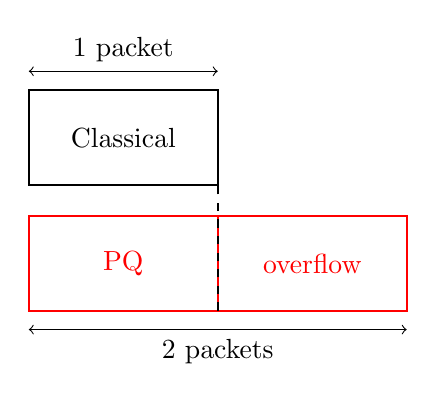
\begin{tikzpicture}[scale=0.8]
					\draw[thick] (0,0) rectangle (3,1.5) node[midway] {Classical};
					\draw[thick,red] (0,-2) rectangle (3,-0.5) node[midway] {PQ};
					\draw[thick,red] (3,-2) rectangle (6,-0.5) node[midway] {overflow};
					\draw[<->] (0,1.8) -- (3,1.8) node[midway,above] {1 packet};
					\draw[<->] (0,-2.3) -- (6,-2.3) node[midway,below] {2 packets};
					\draw[thick,dashed] (3,-2) -- (3,1);
				\end{tikzpicture}
			\end{center}
		\end{column}
	\end{columns}
\end{frame}

\begin{frame}{Current deployment status (2025)}
	\begin{columns}[c]
		\begin{column}{0.6\textwidth}
			\textbf{Browsers have begun implementing PQ TLS:}
			\begin{itemize}
				\item Started with Chrome, now others following
				\item In total, now 38\% of all TLS connection\footnote{\url{https://radar.cloudflare.com/adoption-and-usage\#post-quantum-encryption-adoption}}
			\end{itemize}
			\textbf{Other browsers:}
			\begin{itemize}
				\item Firefox: since mid-2024
				\item Edge, Brave: based on Chrome, so followed it
				\item Safari: timeline announced at WWDC 2025\footnote{\url{https://support.apple.com/en-us/122756}} for iOS 26, macOS 26, etc.
			\end{itemize}
		\end{column}
		\begin{column}{0.4\textwidth}
			\begin{center}
				\textbf{PQ Adoption}\\[3mm]
				\begin{tikzpicture}[scale=0.8]
					\pie[text=legend,radius=2]{
						38/PQ,
						62/Classical
					}
				\end{tikzpicture}
			\end{center}
		\end{column}
	\end{columns}
\end{frame}

\begin{frame}{Beyond browsers: Origin connections}
	\begin{columns}[c]
		\begin{column}{1\textwidth}
			\textbf{The full connection path:}
			\begin{center}
				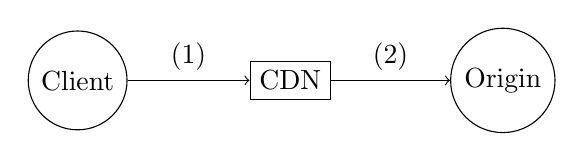
\begin{tikzpicture}[scale=0.9]
					\node[draw,circle] (client) at (0,0) {Client};
					\node[draw,rectangle] (cdn) at (3,0) {CDN};
					\node[draw,circle] (origin) at (6,0) {Origin};
					\draw[->] (client) -- (cdn) node[midway,above] {(1)};
					\draw[->] (cdn) -- (origin) node[midway,above] {(2)};
				\end{tikzpicture}
			\end{center}
			\textbf{Two approaches for CDN-to-origin PQ:}
			\begin{itemize}
				\item \textbf{Fast way}: Send PQ keyshare immediately
				      \begin{itemize}
					      \item Like Chrome's approach
					      \item 0.34\% connection failures observed
				      \end{itemize}
				\item \textbf{Safe way}: Wait for \texttt{HelloRetryRequest}
				      \begin{itemize}
					      \item Extra round trip
					      \item 100\% compatibility
				      \end{itemize}
			\end{itemize}
			\textbf{Failure causes}: Large \texttt{ClientHello} + incorrect \texttt{HelloRetryRequest} handling
		\end{column}
	\end{columns}
\end{frame}

\begin{frame}{Lessons from PQ TLS deployment}
	\begin{itemize}
		\item \textbf{Ossification is real}:
		      \begin{itemize}
			      \item Assumptions about packet sizes break deployments
			      \item GREASE helps but isn't perfect
			      \item Takes years to fix ecosystem
		      \end{itemize}
		\item \textbf{Hybrid approach is prudent}:
		      \begin{itemize}
			      \item Protects against algorithm breaks
			      \item Protects against implementation bugs
			      \item Small performance cost for peace of mind
		      \end{itemize}
		\item \textbf{Deployment is gradual}:
		      \begin{itemize}
			      \item Started in 2016, still ongoing in 2025
			      \item Requires coordination across entire ecosystem
			      \item But progress is accelerating
		      \end{itemize}
	\end{itemize}
\end{frame}

\fi

\subsection{Post-Quantum SSH}

\begin{frame}{OpenSSH: Post-quantum by default}
	\begin{itemize}
		\item \textbf{OpenSSH leading the way}: PQ key agreement by default since 2022
		\item \textbf{Timeline of PQ adoption}:
		      \begin{itemize}
			      \item \textbf{OpenSSH 9.0 (2022)}: First PQ by default
			            \begin{itemize}
				            \item Algorithm: \texttt{sntrup761x25519-sha512}
				            \item Hybrid approach (NTRU + X25519)
			            \end{itemize}
			      \item \textbf{OpenSSH 9.9 (2024)}: Added ML-KEM support
			            \begin{itemize}
				            \item Algorithm: \texttt{mlkem768x25519-sha256}
				            \item Based on NIST standard
			            \end{itemize}
			      \item \textbf{OpenSSH 10.0}: ML-KEM becomes default
			      \item \textbf{OpenSSH 10.1}: Warns on non-PQ connections
		      \end{itemize}
		\item \textbf{The issue}: SSH particularly vulnerable to SNDL (Store Now Decrypt Later)
		      \begin{itemize}
			      \item Entire session privacy depends on key agreement
			      \item Attackers can record SSH sessions today
			      \item Decrypt everything once QC arrives
		      \end{itemize}
	\end{itemize}
\end{frame}

\begin{frame}{OpenSSH's aggressive stance}
	\begin{columns}[c]
		\begin{column}{0.55\textwidth}
			\textbf{The warning (10.1+):}
			\begin{quote}
				\small
				\texttt{** WARNING: connection is not using a post-quantum key exchange algorithm.\\
					** This session may be vulnerable to "store now, decrypt later" attacks.}
			\end{quote}

			\textbf{Why this matters:}
			\begin{itemize}
				\item Pushes ecosystem forward
				\item Makes PQ the norm, not exception
			\end{itemize}
		\end{column}
		\begin{column}{0.45\textwidth}
			\textbf{SSH's unique position:}\footnote{\url{https://www.openssh.com/pq.html}}
			\begin{itemize}
				\item Often used for critical infrastructure
				\item Long-lived connections
				\item High-value targets (admin access)
				\item Perfect for SNDL attacks
			\end{itemize}

			\textbf{Deployment advantage:}
			\begin{itemize}
				\item Simpler than TLS
				\item No certificate chains
				\item Easier to upgrade
			\end{itemize}
		\end{column}
	\end{columns}
\end{frame}

\subsection{The Path Forward}

\begin{frame}{The PQ paradox}
	\begin{itemize}
		\item PQ schemes may initially be LESS secure than classical!
		\item \textbf{Why?}
		      \begin{itemize}
			      \item RSA/ECC: 40 years of implementation hardening
			      \item Constant-time implementations well understood
			      \item Side-channel protections mature
		      \end{itemize}
		\item \textbf{Post-quantum crypto}:
		      \begin{itemize}
			      \item New implementations = new bugs
			      \item Complex operations = more side channels
			      \item Less implementation experience
		      \end{itemize}
		\item \textbf{Timeline of maturity}:
		      \begin{itemize}
			      \item Years 1-5: Discovering vulnerabilities
			      \item Years 5-10: Developing countermeasures
			      \item Years 10+: Mature, hardened implementations
		      \end{itemize}
	\end{itemize}
\end{frame}

\begin{frame}{Lessons learned}
	\begin{itemize}
		\item \textbf{Post-quantum $\neq$ post-security-concerns}
		\item \textbf{Key challenges remain}:
		      \begin{enumerate}
			      \item Unclear concrete security levels
			      \item Implementation vulnerabilities
			      \item Side-channel attacks
			      \item The ``store now, decrypt later'' threat
		      \end{enumerate}
		\item \textbf{Best practices}:
		      \begin{itemize}
			      \item Use conservative parameters
			      \item Implement hybrid solutions (classical + PQ)
			      \item Invest in secure implementations
			      \item Plan for crypto-agility
		      \end{itemize}
	\end{itemize}
\end{frame}

\end{document}